Figure \ref{fig:the proposed approach} shows the proposed approach to the ASL translator. The main approach to developing a translation from American SLA to other SLA is to build the best image recognition model that recognizes each English alphabet from the sign language with high accuracy. Instead of learning from scratch, Transfer learning with pre-trained models, which were already trained on a large benchmark image dataset, can save a lot of computation cost and help the performance. Kera applications provide a wide range of pre-trained models for deep learning such as VGG, ResNet, Xception, etc \cite{keras}. All the available pre-trained models will be applied into the first run training with the partial dataset to find out the Top 5 models with the highest accuracy of prediction. The top 5 models are further optimized and trained with all the training data to determine the best ASL recognition model. In the last phase, the results of prediction are mapping with Turkish ASL images.

\begin{figure}[h]
    \centering
    \caption{The proposed approach for the sign language translator}
	\label{fig:the proposed approach}
    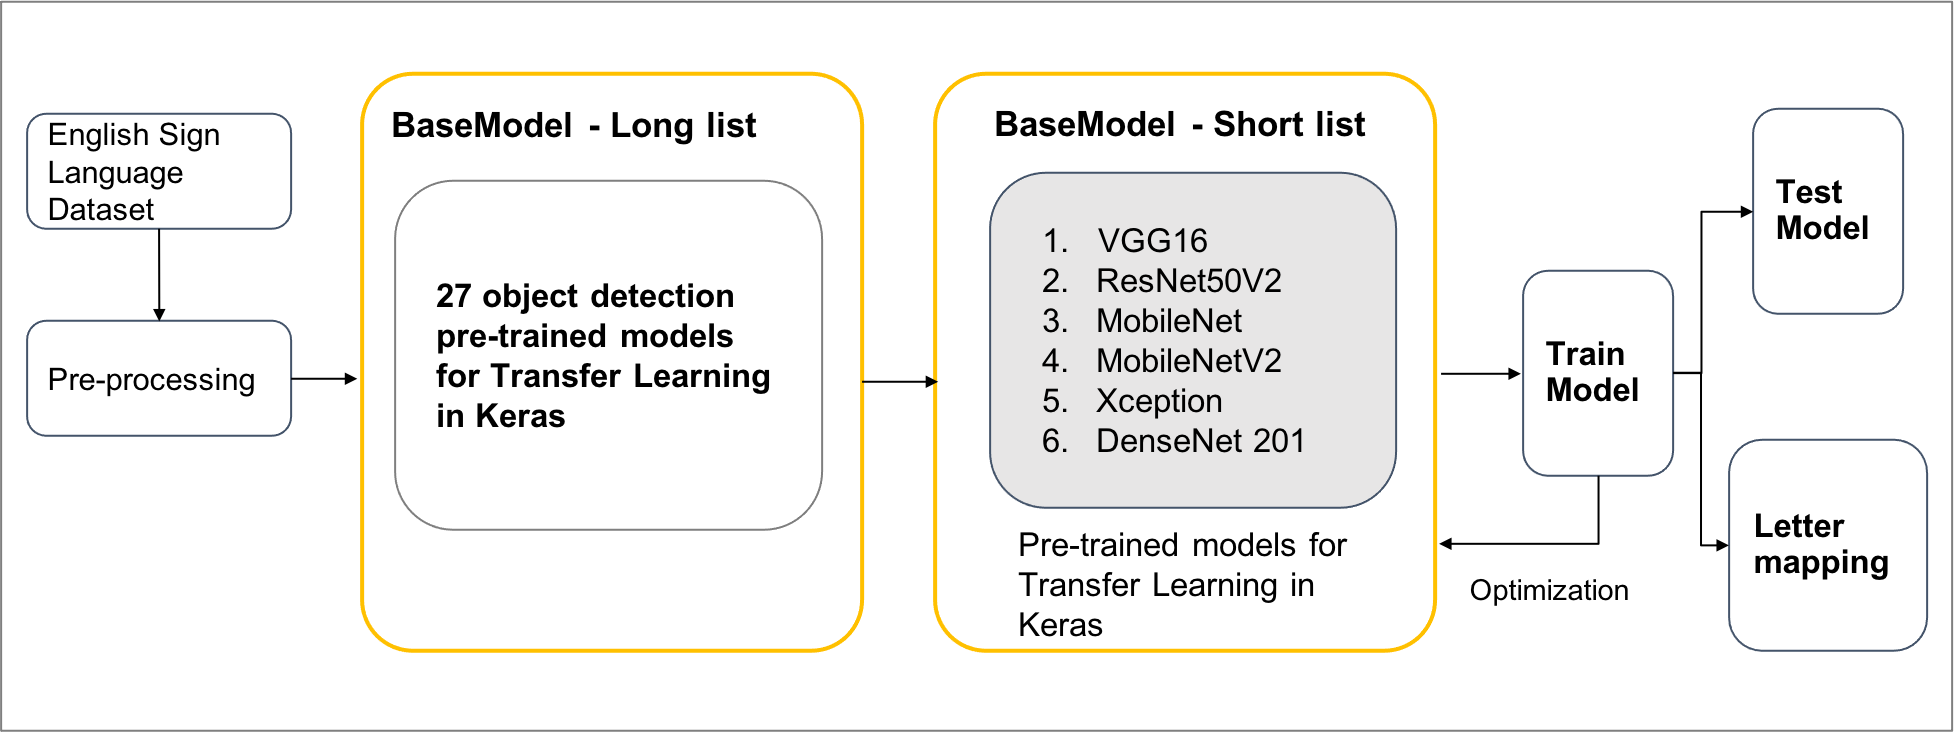
\includegraphics[width=\linewidth]{figures/The approach}
\end{figure}


\subsection{Dataset}
The American ASL dataset is collected from Kaggle. The dataset contains 87,000 images with 26 Englich alphabets and 3 extra signs, which are delete, space, and nothing. All the images are equally distributed to the 29 signs. In other words, each sign has 4,300 images. The whole dataset is split into training and test dataset. Training dataset is 80\% of the data, and the rest data belongs to the test dataset. 


\subsection{Image preprocessing}

\subsection{Transfer learning models}
One of the main benefits of using transfer learning is to make use of previously trained models and save computational cost (CC) for basic tasks like the removal of background. It may also be used when the training data is sparse. For the detection of American SLA we may use (to a degree) any pre-trained model for object detection on our dataset of American SLA signs even if they are limited in count and quality, as they only make the last layer of our final model.

To determine, whether a model may be suitable for our application, we use all of the models and its variants available in Keras\cite{keras}, as shown in Table~\ref{tab:keras_models}. The \textit{Avg. Top-5 Accuracy} in the table refers to the average accuracy of all variants combined.
\begin{table}[th]
    \caption{Keras Applications}
    \label{tab:keras_models}
    \centering
    \begin{tabular}{@{}lrcl@{}}
    \toprule
    Name         & \multicolumn{1}{l}{\begin{tabular}[c]{@{}l@{}}Avg. Top-5\\ Accuracy\end{tabular}} & \multicolumn{1}{l}{Total} & \begin{tabular}[c]{@{}l@{}}Variants\\ (*=Model)\end{tabular}                         \\ \midrule
    Xception     & 0.945                                                                             & 1                         & *                                                                                    \\
    VGG          & 0.901                                                                             & 2                         & *16, *19                                                                             \\
    ResNet       & 0.931                                                                             & 6                         & \begin{tabular}[c]{@{}l@{}}*50, *101, *152,\\  *50V2, *101V2,\\  *152V2\end{tabular} \\
    Inception    & 0.945                                                                             & 2                         & *V3, *ResNetV2                                                                       \\
    MobileNet    & 0.898                                                                             & 2                         & *, *V2                                                                               \\
    DenseNet     & 0.930                                                                             & 3                         & *121, *169, *201                                                                     \\
    NASNet       & 0.940                                                                             & 2                         & *Mobile, *Large                                                                      \\
    EfficientNet & -                                                                                 & 8                         & \begin{tabular}[c]{@{}l@{}}*B0, *B1, *B2,\\  *B3, *B4, *B5,\\  *B6, *B7\end{tabular} \\ \bottomrule
    \end{tabular}
\end{table}

In order to determine, which of the above stated models we will further evaluate and possibly optimize, we train each of the Keras models in an experimental setup. The experimental training is defined by:
\begin{enumerate}
    \item Training with 5\% of the dataset (~4.300 images, equally distributed to the 29 targets), with a 80/20 Train-Test-Split
    \item 10 Epochs of Training
    \item No Early Stopping
\end{enumerate}

The results will focus on two key indicators: accuracy on our dataset and training time.

The following subsections will give a brief introduction of the most relevant model families and how they differ.

\subsubsection{VGG16}
The VGG models are one of the earlier computer vision models an were introduced in 2015 by Simonyan and Zisserman which showed that using deep architectures with rather small filters can be superior to other models at that time\cite{simonyan2015deep}. VGG represents a classical convolutional neural network which takes an 224x224x3 (width x height x channels) input pictures and passes it to multiple convolutional layers, pooling layers and activation functions to a fully connected final layer for classification. It includes in total 16 layers with weights and is shown in figure \ref{fig:vgg16}.

\begin{figure}
  \centering
  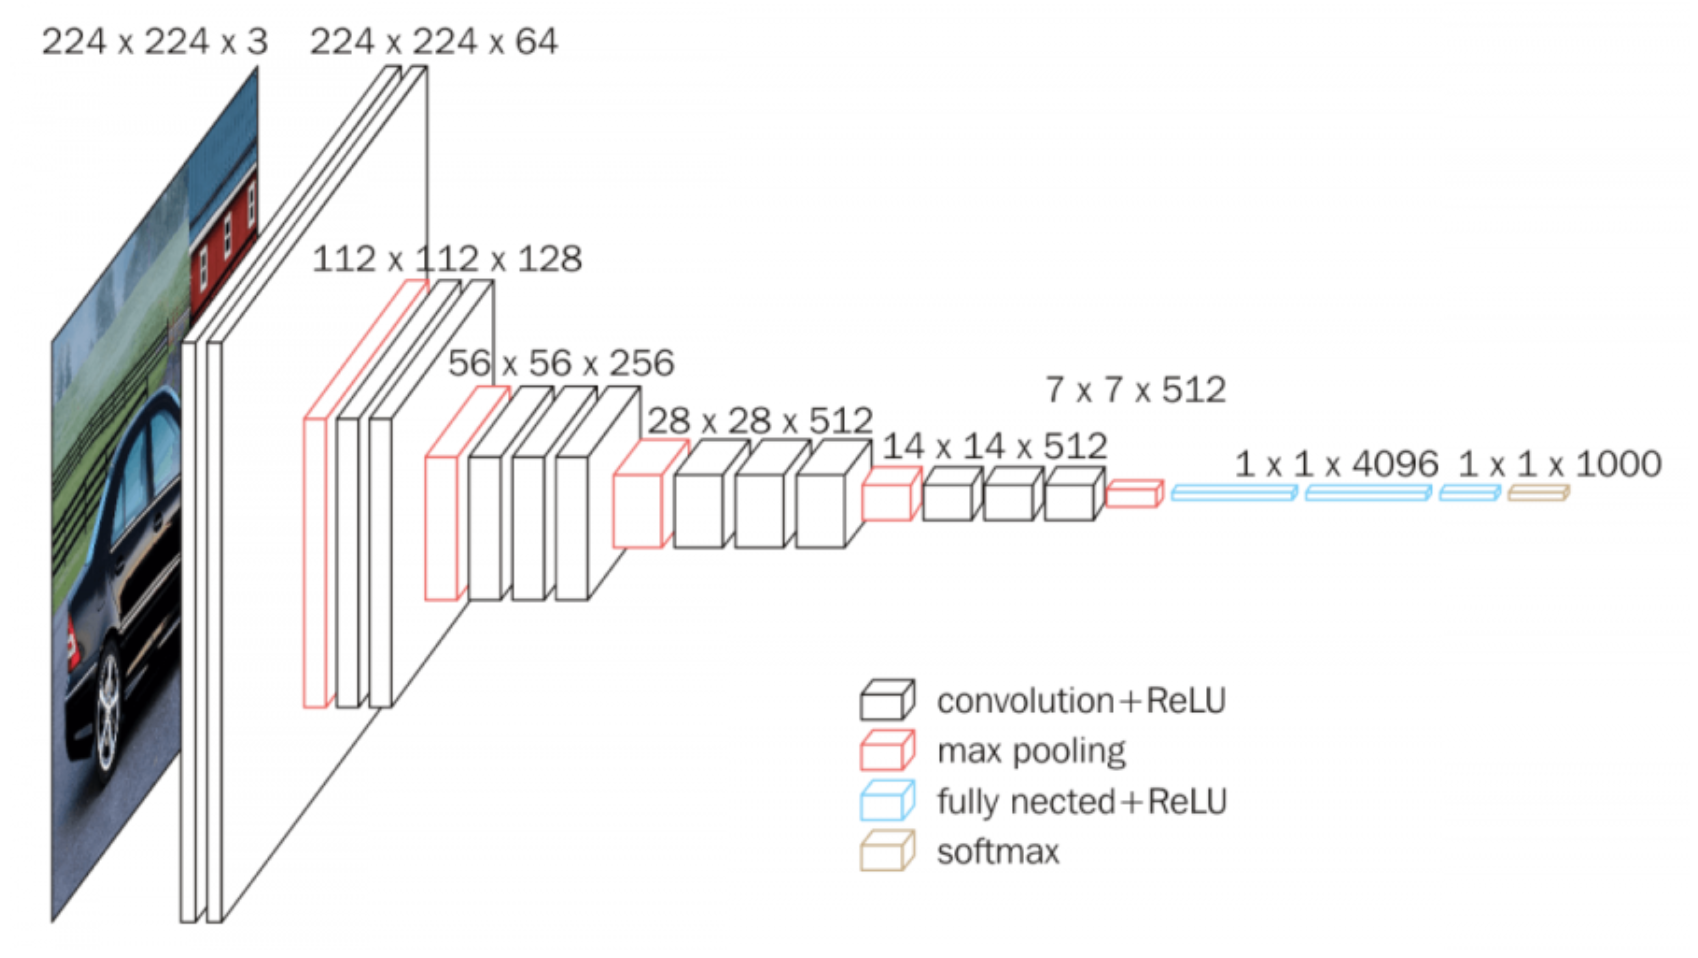
\includegraphics[width=\linewidth]{figures/vgg16.png}
  \caption{VGG16 architecture}
  \label{fig:vgg16}
\end{figure}

The tremendous change compared to previous convolutional neural networks is that the used filters and layers have the same size and parameters such as only ReLu as activation function\cite{simonyan2015deep}. This newly introduced simplicity paired with a relatively deep architecture led to unique results in the ILSVRC-2012 and ILSVRC-2013 competitions compared to the previous state-of-art AlexNet. On top of that is was shown that the model had a strong ability to generalise over multiple datasets and still achieve a top 5 performance. The authors of the network structured it in a way that it is possible to move from 16 layers to 19 layers for even better results.

\subsubsection{ResNet50V2}\label{resnet}
Due to the fact that the performance of very deep neural network started to decrease at some point and while backpropagating the vanishing gradient became another problem, He et al. introduced the "residual units" for the new architecture\cite{he2015deep}. The main idea is to not only pass processed information from layer to layer but also to layers further ahead in the network. This skipping of e.g. one layer has been introduced as "skip-connection" or "identity shortcut". The layers and its connections to other layers are arranged as residual blocks which share the same input and output size within the block\cite{he2015deep}. The connection from one block to another is done by a "projection shortcut" which allows a change in input and output dimensions.

\begin{figure}
  \centering
  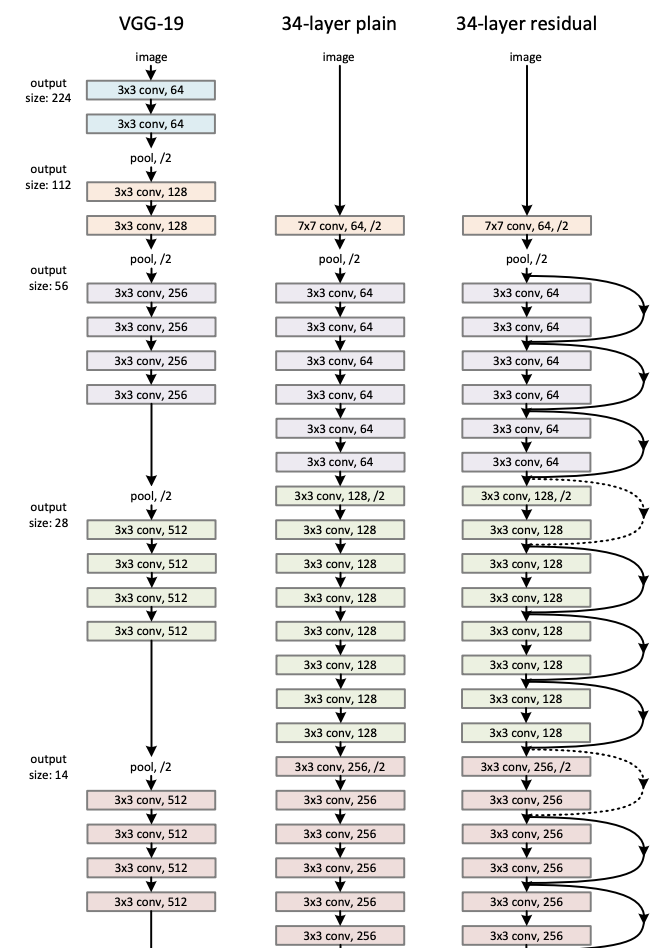
\includegraphics[width=\linewidth]{figures/resnet.png}
  \caption{ResNet architecture}
  \label{fig:resnet}
\end{figure}

Figure \ref{fig:resnet} presents the individual residual units on the right side distinguished by the color. The dotted connections represent the projection shortcuts whereas the solid arrows represent the identity shortcuts.
This newly introduced architecture enabled the authors to solve both of the above mentioned issues and build deep, high performing neural networks. The main reason of this achievement is that higher layers can learn important information from the lower layers directly.

\subsubsection{MobileNet}\label{mobilenet}

MobileNet was developed by Google Inc. with the purpose to be used for mobile and embedded vision applications. This target leads to the fact that the model has been optimised for latency.
The authors introduced "depthwise separable convolutions" in which the channels are separately convoluted on their on an combined through a 1x1 pointwise convolution\cite{howard2017mobilenets}. A visualisation can be found in figure\ref{fig:mobilenet}. This separation of the convolution for each channel and a followed combination of thee feature map results in significantly less computation than compared to the previous neural networks and therefore minimises the latency drastically by appx. 8 times\cite{howard2017mobilenets}.

\begin{figure}
  \centering
  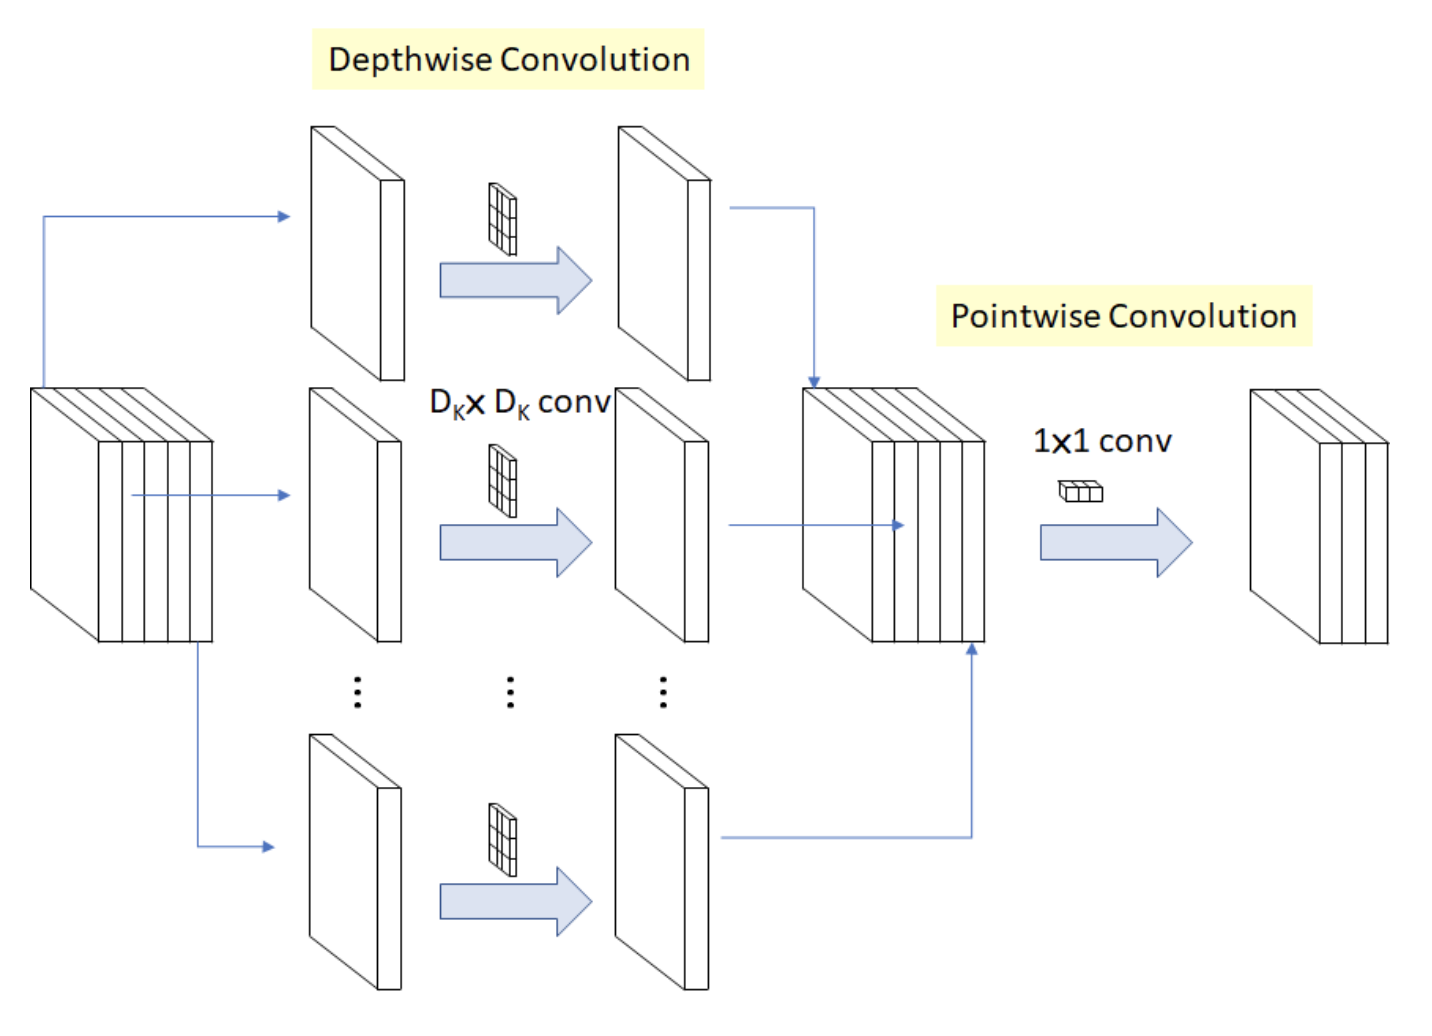
\includegraphics[width=\linewidth]{figures/mobilenet.png}
  \caption{MobileNet architecture}
  \label{fig:mobilenet}
\end{figure}

Besides the tremendous success with focus and latency such as a high performance on the usual benchmark datasets for e.g. facial recognition, the authors found out that with this approach less regularisation and data augmentation is needed to achieve state-of-art results.

\subsubsection{MobileNetV2}
The second version of the MobileNet introduces two additions to its predecessor. The first one is called bottleneck layer where a a lowdimensional feature vector is passed to the respective layer which then expands this vector to a highdimensional space, applies a depthwise convolution and reduces the dimensions again to deliver the output\cite{sandler2019mobilenetv2}. This way the number of computations through out the entire network are kept stable which has a positive impact on the latency. As this technique leads to some loss of contained information the authors introduced residual units which follow the same logic like the units explained in section \ref{resnet}. This way information can be passed by skipping a layer and the information loss due to the bottleneck layer is reduced.

\begin{table}[th]
    \caption{MobileNet comparison}
    \label{tab:mobilenet_comparision}
    \centering
    \begin{tabular}{@{}lrcl@{}}
    \toprule
    Version         & \multicolumn{1}{l}{\begin{tabular}[c]{@{}l@{}}MACs (millions)\end{tabular}} & \multicolumn{1}{l}{Parameters (millions)}                        \\ \midrule
    MobileNetV1     & 569                                                                             & 4.24                                                                                 \\
    MobileNetV2          & 300                                                                             & 3.47\end{tabular}
\end{table}

\begin{table}[th]
    \caption{MobileNet FPS comparison}
    \label{tab:mobilenet_fps_comparision}
    \centering
    \begin{tabular}{@{}lrcl@{}}
    \toprule
    Version         & \multicolumn{1}{l}{\begin{tabular}[c]{@{}l@{}}iPhone 7)\end{tabular}} & \multicolumn{1}{l}{iPhone X)}& \multicolumn{1}{l}{iPad Pro 10.5)}                        \\ \midrule
    MobileNetV1     & 118                                                                             & 162 & 204                                                                                \\
    MobileNetV2          & 145                                                                             & 233 & 220\end{tabular}
\end{table}

Additionally the authors showed an increased performance on benchmark datasets such as a potential combination with single shot detection (SSD) which can yield into even better and faster results.

\subsubsection{DenseNet 201}

Dense convolutional networks, also called DenseNet, were introduced in 2016 by Huang et al. and proposed a new way of building very deep neural networks which are stable to train and high performing. The change compared to other architectures was that each layer is connected to all following layers to pass the resulting feature vector through the entire network\cite{huang2018densely}. A visual illustration can be found in figure \ref{densnet}.

\begin{figure}
  \centering
  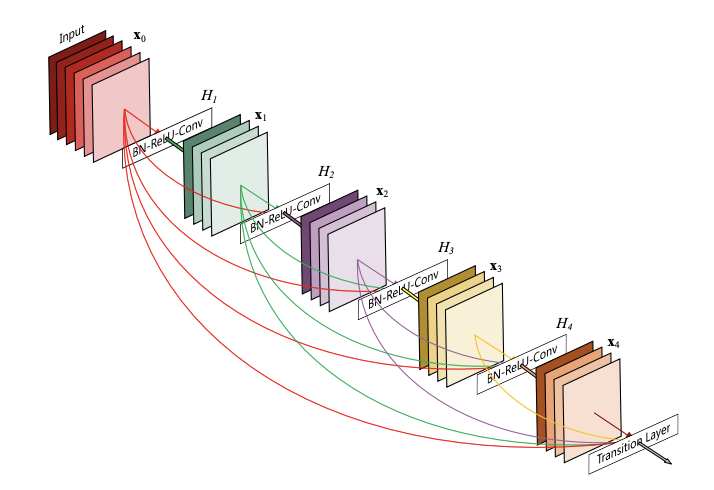
\includegraphics[width=\linewidth]{figures/densenet.png}
  \caption{DensNet architecture}
  \label{densnet}
\end{figure}

The connection from one layer to all following layers is in a typical fast-forward manner which leads to the following advantages:
\begin{itemize}
  \item alleviate the vanishing-gradient problem
  \item stronger feature re-use
  \item smaller number of parameters
\end{itemize}

The reduced number of parameters is a result of the network being able to ignore redundant feature maps which do not need to be learned again. In the initial paper the authors propose an architecture with very narrow layers (12 filters per layer)\cite{huang2018densely}. Due to the complete connection of all layers the model is less likely to overfit and more stable to train.
The model contains residual units as well which shall strengthen the information flow from previous to later layers. Additionally bottleneck layers can be found which were introduced to minimise the number of computations being caused by the complex connectivity.

\subsubsection{Xception}

Xception is an advanced version of Google's Inception model and a short form of "Extreme Inception". The previous architecture of Inception convoluted the input channel by channel and combined the results in the end. This depthwise separable convolution was slightly modified in newly introduced Xception model by Chollet\cite{chollet2017xception}. The author changed the regular set up of first applying a depthwise convolution and then the pointwise to a set up which executes these steps the other way round. However this change only did not lead to major improvements with regard to performance which is why a second change was applied by introducing residual connections\cite{chollet2017xception}.
\begin{figure}
  \centering
  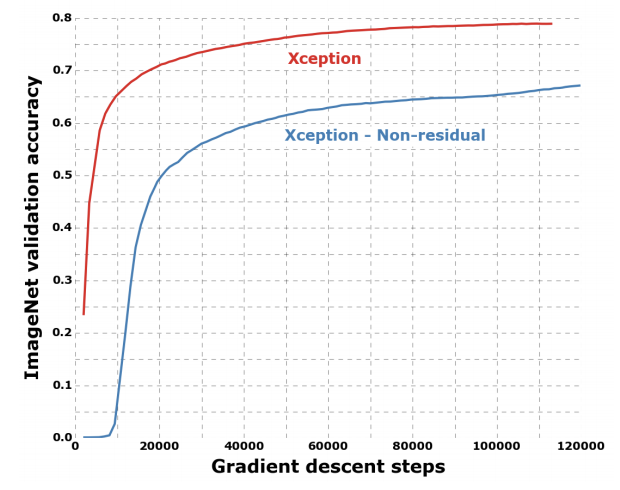
\includegraphics[width=\linewidth]{figures/xception_residuals.png}
  \caption{Impact of residual units for Xception}
  \label{xception_residuals}
\end{figure}

Figure \ref{xception_residuals} shows a clear improvement of the introduction of residual blocks.

Furthermore the author removed the ReLu activation after the depthwise convolution, different than in the Inception architecture, which had a tremendous impact on the model performance.
\begin{figure}
  \centering
  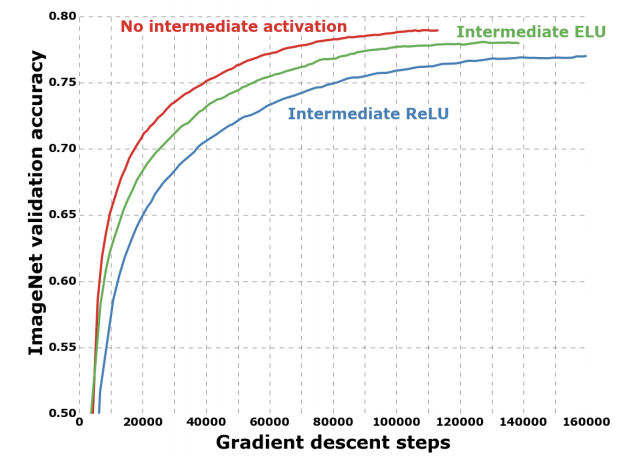
\includegraphics[width=\linewidth]{figures/xception_activation.png}
  \caption{Impact of removing ReLu activation}
  \label{xception_activation}
\end{figure}

The above mentioned changes not only led to a similar model size like Inception-V3 but also outperform  VGGNet, ResNet, and Inception-v3 in accuracy with regard to known benchmark datasets\cite{chollet2017xception}.


